\documentclass[11pt,a4paper]{article}
\usepackage[utf8]{inputenc}
\usepackage[T1]{fontenc}
\usepackage{lmodern}
\usepackage{microtype}
\usepackage{amsmath,amssymb,amsfonts}
\usepackage{enumitem}
\usepackage{bm}
\usepackage{graphicx}
\usepackage{booktabs}
\usepackage{caption}
\usepackage[margin=2.5cm]{geometry}
\usepackage{setspace}
\onehalfspacing
\usepackage{titletoc}
\usepackage{fancyhdr}
\usepackage[colorlinks=true,linkcolor=black,citecolor=black,urlcolor=blue]{hyperref}
\usepackage{placeins}
\usepackage[capitalise,nameinlink]{cleveref}
\usepackage{tikz}
%---------------------- Custom macros (identical to the main report) -----
\newcommand{\conc}{c}
\newcommand{\Cd}[2]{C_{#1}^{#2}}
\newcommand{\pd}[2]{\frac{\partial #1}{\partial #2}}
\newcommand{\pdd}[2]{\frac{\partial^{2} #1}{\partial #2^{2}}}
\newcommand{\Lap}{\nabla^{2}}
\newcommand{\dr}{\Delta r}
\newcommand{\dt}{\Delta t}
\newcommand{\Fo}{\mathrm{Fo}}
\newcommand{\Diff}{D}
\newcommand{\decayrate}{\lambda}
\newcommand{\fissxs}{\Sigma_{f}}
\newcommand{\flux}{\phi}
\newcommand{\yield}{Y}
\newcommand{\trap}{\kappa}
\newcommand{\Bi}{\mathrm{Bi}}
\newcommand{\dd}{\,\mathrm{d}}
\pagestyle{fancy}
\fancyhf{}
\fancyhead[L]{\small Hand-Derived Analytical Solutions --- Submission to Theodore}
\fancyhead[R]{\small \thepage}
\renewcommand{\headrulewidth}{0.2pt}
\title{\bfseries Hand-Derived Analytical Solutions\\[0.3em]
\large Fission-Product Diffusion in TRISO Fuel Particles\\[0.3em]
\normalsize Submission to Theodore}
\author{Ray~W.}
\date{\today}
\begin{document}
\maketitle
\begin{abstract}
This file reproduces, in LaTeX, the equations and derivations from the TRISO
fuel particle diffusion analysis that were derived independently by the
author. It is a narrower excerpt of the full consolidated reference
(\texttt{equations/all\_equations.tex}) in this repository: the Arrhenius
temperature-dependence relation, the completed eigenvalue problem and
closed-form series solution beyond the raw eigencondition, and the
five-layer multilayer particle model are all omitted here, since none of
them were developed by the author personally. What remains is the physical
system, the governing equation and its assumptions, and the homogeneous
single-sphere (Part I) analytical derivation through the raw eigencondition,
together with its FTCS numerical discretisation. Notation, variables, and
units are defined in the Reference Frame below; every equation is numbered
automatically and, where it also appears in the main report, carries the
identical \texttt{\textbackslash label} so the two documents cross-reference
unambiguously.
\end{abstract}
\tableofcontents
\clearpage

\section*{The Physical System}
\addcontentsline{toc}{section}{The Physical System}
\begin{figure}[htbp]
  \centering
  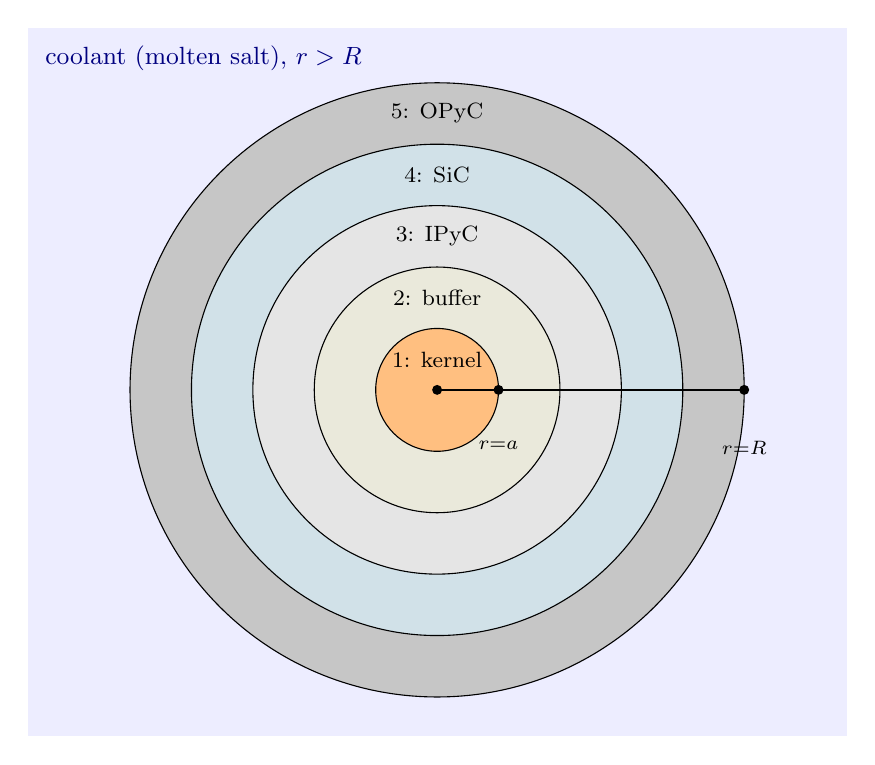
\begin{tikzpicture}[scale=1.0, >=latex, font=\small]
    \fill[blue!7] (-5.2,-4.4) rectangle (5.2,4.6);
    \node[anchor=north west, blue!50!black] at (-5.1,4.5)
      {coolant (molten salt), $r > R$};
    \fill[gray!45]           (0,0) circle (3.9);
    \fill[cyan!35!gray!30]   (0,0) circle (3.12);
    \fill[gray!20]           (0,0) circle (2.34);
    \fill[yellow!25!gray!25] (0,0) circle (1.56);
    \fill[orange!50]         (0,0) circle (0.78);
    \draw[thin] (0,0) circle (0.78);
    \draw[thin] (0,0) circle (1.56);
    \draw[thin] (0,0) circle (2.34);
    \draw[thin] (0,0) circle (3.12);
    \draw[thin] (0,0) circle (3.9);
    \node[font=\footnotesize] at (0,0.38)  {1: kernel};
    \node[font=\footnotesize] at (0,1.17)  {2: buffer};
    \node[font=\footnotesize] at (0,1.95)  {3: IPyC};
    \node[font=\footnotesize] at (0,2.73)  {4: SiC};
    \node[font=\footnotesize] at (0,3.51)  {5: OPyC};
    \draw[thick] (0,0) -- (3.9,0);
    \fill (0,0) circle (1.8pt);
    \fill (0.78,0) circle (1.8pt);
    \fill (3.9,0) circle (1.8pt);
    \node[below=15pt] at (0.78,0) {\scriptsize $r{=}a$};
    \node[below=15pt] at (3.9,0)  {\scriptsize $r{=}R$};
  \end{tikzpicture}
  \caption{The idealised five-layer TRISO particle modelled in this
  reference: fuel kernel (layer 1, $0\le r\le a$, where the volumetric source
  $S_0$ acts), buffer, IPyC, and SiC (layers 2 to 4), and OPyC (layer 5, outer
  radius $R$). Coolant flows past the particle at $r>R$ and is treated as a
  finite-resistance convective (Robin) boundary at $r=R$ throughout, rather
  than an idealised perfect sink. Part I collapses all five layers into a
  single homogeneous region of shared diffusivity $D$, shown here; Part II
  resolves the five physical layers individually, assigning each shell its
  own diffusivity $D_i$. Shell thicknesses are drawn equal for legibility;
  real layer thicknesses differ. Not to scale. Adapted from the system
  diagram in the main report
  (\texttt{report/sections/02\_system\_overview.tex}).}
  \label{fig:eq-particle}
\end{figure}
\FloatBarrier
\clearpage

\section*{Reference Frame}
\addcontentsline{toc}{section}{Reference Frame}

\begin{center}
\small
\begin{tabular}{@{}lp{9.3cm}l@{}}
\toprule
Symbol & Definition & Units \\
\midrule
$c(r,t)$       & Concentration of the diffusing fission-product species & $\mathrm{mol\ m^{-3}}$ \\
$\Cd{i}{j}$    & Discrete concentration at node $i$, time level $j$ (FTCS) & $\mathrm{mol\ m^{-3}}$ \\
$t$            & Time                                                  & $\mathrm{s}$ \\
$r$            & Radial coordinate                                     & $\mathrm{m}$ \\
$a$, $r_1$     & Kernel (layer 1) outer radius (used interchangeably)  & $\mathrm{m}$ \\
$R$            & Particle outer radius (OPyC/coolant surface)          & $\mathrm{m}$ \\
$D$, $D_i$     & Diffusivity (Part I: single shared value; Part II: layer $i$) & $\mathrm{m^{2}\ s^{-1}}$ \\
$S$, $S_{0}$   & Volumetric source/sink term; kernel source strength    & $\mathrm{mol\ m^{-3}\ s^{-1}}$ \\
$h$            & Convective mass-transfer coefficient at the surface   & $\mathrm{m\ s^{-1}}$ \\
$\Bi$          & Biot number, $hR/D$ (Part I) or $hR/D_L$ (Part II)    & --- \\
$\dr$          & Radial mesh spacing                                   & $\mathrm{m}$ \\
$\dt$          & Time-step size                                        & $\mathrm{s}$ \\
$i,j$          & Radial node index; time-level index                   & --- \\
$N$            & Index of the surface node (mesh-cell count, centre to surface) & --- \\
$\Fo$          & Mesh Fourier number, $\Diff\dt/\dr^{2}$               & --- \\
$\kappa$       & Mesh-local convective ratio, $h\dr/D=\Bi/N$           & --- \\
$D_k^{\mathrm{eff}}$ & Effective diffusivity at an interface node (Part II FTCS) & $\mathrm{m^{2}\ s^{-1}}$ \\
$w(r)$         & Steady-state concentration profile                    & $\mathrm{mol\ m^{-3}}$ \\
$\phi_n(r)$    & $n$-th eigenfunction, $u_n(r)/r$                      & $\mathrm{m^{-1}}$ \\
$\mu_n$        & Dimensionless root of the Part I eigencondition $\mu\cot\mu=1-\Bi$ & --- \\
$\lambda_n$    & Modal decay rate (eigenvalue) of mode $n$; $\lambda_n\equiv D\mu_n^2/R^2$ in Part I & $\mathrm{s^{-1}}$ \\
$N_n$          & Normalisation integral, $\int_0^R \phi_n^2 r^2\,\dd r$ & $\mathrm{m^{3}}$ \\
$a_n$, $b_n$   & Expansion coefficients (source-active; post-shutdown) & $\mathrm{mol\ m^{-2}}$ \\
$t_c$          & Time at which the source is switched off (shutdown)   & $\mathrm{s}$ \\
$P_i$, $J_i$   & Layer propagator matrix; interface jump matrix, $\det=1$ (Part II) & --- \\
$F(\lambda)$   & Eigencondition function whose positive roots are the $\lambda_n$ (Part II) & --- \\
$\rho_i$       & Shell resistance of layer $i$, $\frac{1}{4\pi D_i}\left(\frac1{r_{i-1}}-\frac1{r_i}\right)$ & $\mathrm{s\ m^{-3}}$ \\
\bottomrule
\end{tabular}
\end{center}
\clearpage

\section*{Assumptions}
\addcontentsline{toc}{section}{Assumptions}

Before any equation is written down, five standing physical assumptions fix
the scope of this model. Each is invoked explicitly at the point in the
derivation where it does the work of turning a general statement into a
solvable one.

\begin{description}
  \item[Assumption 1 (spherical uniformity).] The kernel composition and the
  species source are uniform over each spherical shell, so the concentration
  field depends on the radial coordinate $r$ and time $t$ alone, never on the
  polar or azimuthal angle. This is what collapses the full spherical
  diffusion equation to one radial dimension in the Governing Equation
  section below.
  \item[Assumption 2 (a single representative particle).] The model
  describes one particle in isolation, driven by a specified kernel source
  and a specified coolant-side condition; it does not resolve
  particle-to-particle variability, particle packing in the fuel compact, or
  the coolant-side thermal-hydraulic field that would set $h$ in a
  full-core calculation. Those quantities are treated as given inputs.
  \item[Assumption 3 (kernel-confined source).] Fission events, and with them
  the fission-product species being tracked, occur only inside the fissile
  kernel. The buffer, IPyC, SiC, and OPyC layers contain no fissile
  material, so the volumetric source term is exactly zero there.
  \item[Assumption 4 (piecewise-uniform diffusivity, ideal interfacial
  contact).] Each layer is modelled as a distinct homogeneous material with
  its own diffusivity, so nothing forces the diffusivity itself to be
  continuous from one layer to the next. What does hold, assuming ideal
  contact between adjacent shells with no additional interfacial resistance,
  is that the concentration itself does not jump and that whatever flux
  leaves one layer enters the next.
  \item[Assumption 5 (convective surface condition).] The coolant is a
  finite, well-mixed reservoir that removes the diffusing species at a rate
  proportional to how far the surface concentration sits above the
  coolant's own concentration, rather than instantly to zero. This
  convective (Robin) condition is the physically realistic representation of
  a real coolant with finite mass-transfer resistance; an idealised perfect
  sink is the $\Bi\to\infty$ limiting case of it.
\end{description}

Part I below adopts a further simplification of its own, a
uniform-everywhere source in place of Assumption 3's kernel-confined one, in
exchange for a fully analytical solution.
\clearpage


\section{Initial and Boundary Conditions}
\label{sec:icbc}

The initial condition and boundary conditions close the governing equation
once its form is fixed, before any particular solution technique is
applied. The centre condition follows from Assumption 1: spherical symmetry
rules out a kink in the concentration field at the coordinate singularity
$r=0$, so its radial derivative there must vanish. The outer condition
follows from Assumption 5, the convective surface: the flux leaving the
particle is proportional to how far the surface concentration sits above
the (zero) coolant concentration, rather than being fixed outright. The
initial condition reflects a freshly fabricated particle carrying none of
the diffusing species yet.

\begin{align}
c(r,0) &= 0, \label{eq:b:ic}\\
\frac{\partial c}{\partial r}(0,t) &= 0 \quad\text{(spherical symmetry, Assumption 1)}, \label{eq:b:bc0}\\
-D\frac{\partial c}{\partial r}(R,t) &= h\,c(R,t) \quad\text{(convective release, Assumption 5)}. \label{eq:b:bcR}
\end{align}
\vspace{-0.3em}
\noindent where:

\begin{itemize}[leftmargin=1.6em,itemsep=1pt,topsep=3pt,parsep=0pt]
  \item $c(r,0)$ = initial concentration field ($\mathrm{mol\,m^{-3}}$);
  \item $r$ = radial coordinate ($\mathrm{m}$);
  \item $t$ = time ($\mathrm{s}$);
  \item $D$ = diffusivity ($\mathrm{m^{2}\,s^{-1}}$);
  \item $R$ = particle outer radius ($\mathrm{m}$);
  \item $h$ = convective mass-transfer coefficient at the surface ($\mathrm{m\,s^{-1}}$);
  \item $c(R,t)$ = surface concentration ($\mathrm{mol\,m^{-3}}$).
\end{itemize}

\paragraph{Biot number.}

\begin{equation}
\Bi = \frac{hR}{D},
\label{eq:b:biot}
\end{equation}
\vspace{-0.3em}
\noindent where:

\begin{itemize}[leftmargin=1.6em,itemsep=1pt,topsep=3pt,parsep=0pt]
  \item $\mathrm{Bi}$ = Biot number, ratio of surface convective transport to internal diffusive transport (dimensionless);
  \item $h$ = convective mass-transfer coefficient ($\mathrm{m\,s^{-1}}$);
  \item $R$ = particle outer radius ($\mathrm{m}$);
  \item $D$ = diffusivity ($\mathrm{m^{2}\,s^{-1}}$).
\end{itemize}
\clearpage

\section{The Governing Equation}
\label{sec:governing-equation}


\paragraph{Fick's second law with a volumetric source term (general form).}

\begin{equation}
  \pd{\conc}{t} = \Diff \, \Lap \conc + S ,
  \label{eq:fick}
\end{equation}
\vspace{-0.3em}
\noindent where:

\begin{itemize}[leftmargin=1.6em,itemsep=1pt,topsep=3pt,parsep=0pt]
  \item $c$ = concentration of the diffusing fission-product species ($\mathrm{mol\,m^{-3}}$);
  \item $t$ = time ($\mathrm{s}$);
  \item $D$ = diffusion coefficient ($\mathrm{m^{2}\,s^{-1}}$);
  \item $\nabla^{2}$ = Laplacian (divergence-of-gradient) operator ($\mathrm{m^{-2}}$);
  \item $S$ = volumetric source/sink term ($\mathrm{mol\,m^{-3}\,s^{-1}}$).
\end{itemize}



\paragraph{Fick's second law in spherical coordinates.}

\begin{equation}
  \pd{\conc}{t}
  = \Diff \left[
      \frac{1}{r^{2}} \pd{}{r}\!\left( r^{2}\,\pd{\conc}{r} \right)
      + \frac{1}{r^{2}\sin\theta} \pd{}{\theta}\!\left( \sin\theta \, \pd{\conc}{\theta} \right)
      + \frac{1}{r^{2}\sin^{2}\theta} \pdd{\conc}{\varphi}
    \right] + S .
  \label{eq:fick-spherical}
\end{equation}
\vspace{-0.3em}
\noindent where:

\begin{itemize}[leftmargin=1.6em,itemsep=1pt,topsep=3pt,parsep=0pt]
  \item $c$ = concentration field ($\mathrm{mol\,m^{-3}}$);
  \item $t$ = time ($\mathrm{s}$);
  \item $D$ = diffusion coefficient ($\mathrm{m^{2}\,s^{-1}}$);
  \item $r$ = radial coordinate ($\mathrm{m}$);
  \item $\theta$ = polar (colatitude) angle ($\mathrm{rad}$);
  \item $\varphi$ = azimuthal angle ($\mathrm{rad}$);
  \item $S$ = volumetric source/sink term ($\mathrm{mol\,m^{-3}\,s^{-1}}$).
\end{itemize}



\paragraph{Reduction to one radial dimension (spherical uniformity, Assumption 1).}
The TRISO particle is built from concentric, materially uniform shells, and both the source term and the diffusivity in \cref{eq:fick-spherical} depend on $r$ alone, so nothing in the geometry or the physics picks out one polar or azimuthal direction over another. The concentration field inherits that symmetry, $c=c(r,t)$, so $\partial c/\partial\theta=\partial c/\partial\varphi=0$ and the two angular terms in \cref{eq:fick-spherical} vanish identically. What is left is a genuinely one-dimensional problem in $r$ alone:

\begin{equation}
  \pd{\conc}{t}
  = \Diff \left[ \frac{1}{r^{2}} \pd{}{r}\!\left( r^{2}\,\pd{\conc}{r} \right) \right]
  + S(r,t).
  \label{eq:radial-conservative}
\end{equation}
\vspace{-0.3em}
\noindent where:

\begin{itemize}[leftmargin=1.6em,itemsep=1pt,topsep=3pt,parsep=0pt]
  \item $c$ = concentration field, now a function of $r,t$ only under spherical symmetry ($\mathrm{mol\,m^{-3}}$);
  \item $t$ = time ($\mathrm{s}$);
  \item $D$ = diffusion coefficient ($\mathrm{m^{2}\,s^{-1}}$);
  \item $r$ = radial coordinate ($\mathrm{m}$);
  \item $S(r,t)$ = volumetric source/sink term ($\mathrm{mol\,m^{-3}\,s^{-1}}$).
\end{itemize}



\paragraph{Expansion of the conservative flux term.}

\begin{equation}
  \frac{1}{r^{2}} \pd{}{r}\!\left( r^{2}\,\pd{\conc}{r} \right)
  = \frac{1}{r^{2}} \left[ 2r\,\pd{\conc}{r} + r^{2}\,\pdd{\conc}{r} \right]
  = \pdd{\conc}{r} + \frac{2}{r}\,\pd{\conc}{r},
  \label{eq:product-rule}
\end{equation}
\vspace{-0.3em}
\noindent where:

\begin{itemize}[leftmargin=1.6em,itemsep=1pt,topsep=3pt,parsep=0pt]
  \item $c$ = concentration field ($\mathrm{mol\,m^{-3}}$);
  \item $r$ = radial coordinate ($\mathrm{m}$).
\end{itemize}



\paragraph{The governing equation used throughout this reference.}

\begin{equation}
  \boxed{\;
  \pd{\conc}{t}
  = \Diff \left( \pdd{\conc}{r} + \frac{2}{r}\,\pd{\conc}{r} \right) + S(r,t).
  \;}
  \label{eq:simplified-triso}
\end{equation}
\vspace{-0.3em}
\noindent where:

\begin{itemize}[leftmargin=1.6em,itemsep=1pt,topsep=3pt,parsep=0pt]
  \item $c$ = concentration field ($\mathrm{mol\,m^{-3}}$);
  \item $t$ = time ($\mathrm{s}$);
  \item $D$ = diffusion coefficient ($\mathrm{m^{2}\,s^{-1}}$);
  \item $r$ = radial coordinate ($\mathrm{m}$);
  \item $S(r,t)$ = volumetric source/sink term ($\mathrm{mol\,m^{-3}\,s^{-1}}$).
\end{itemize}



\paragraph{Kernel-localised volumetric source term (Assumption 3).}
Fission events, and with them the generation of the fission-product species being tracked, occur only inside the fissile kernel. The buffer, IPyC, SiC, and OPyC layers contain no fissile material, so $S(r)$ is exactly zero there regardless of how each layer's diffusivity is modelled. This is a statement about where the species is created, not a simplifying approximation:

\begin{equation}
  S(r) =
  \begin{cases}
    S_0, & 0 \le r \le a \quad \text{(layer 1, kernel)}, \\
    0,   & a < r \le R \quad \text{(layers 2--5, buffer and coatings)},
  \end{cases}
  \label{eq:kernel-source}
\end{equation}
\vspace{-0.3em}
\noindent where:

\begin{itemize}[leftmargin=1.6em,itemsep=1pt,topsep=3pt,parsep=0pt]
  \item $S(r)$ = volumetric source term at radius $r$ ($\mathrm{mol\,m^{-3}\,s^{-1}}$);
  \item $S_0$ = kernel source strength ($\mathrm{mol\,m^{-3}\,s^{-1}}$);
  \item $r$ = radial coordinate ($\mathrm{m}$);
  \item $a$ = kernel (layer 1) outer radius ($\mathrm{m}$);
  \item $R$ = particle outer radius ($\mathrm{m}$).
\end{itemize}



\section{Physical Models for the Source Term and Diffusion Coefficient}
\label{sec:source-terms}

\paragraph{Decomposition of the volumetric source term.}

\begin{equation}
  S(\conc, r, t) = S_{\text{gen}} + S_{\text{decay}} + S_{\text{trap}} ,
  \label{eq:source-decomposition}
\end{equation}
\vspace{-0.3em}
\noindent where:

\begin{itemize}[leftmargin=1.6em,itemsep=1pt,topsep=3pt,parsep=0pt]
  \item $S(c,r,t)$ = total volumetric source term ($\mathrm{mol\,m^{-3}\,s^{-1}}$);
  \item $S_{\text{gen}}$ = generation term from fission ($\mathrm{mol\,m^{-3}\,s^{-1}}$);
  \item $S_{\text{decay}}$ = radioactive-decay loss term ($\mathrm{mol\,m^{-3}\,s^{-1}}$);
  \item $S_{\text{trap}}$ = trapping/release term ($\mathrm{mol\,m^{-3}\,s^{-1}}$);
  \item $c$ = concentration ($\mathrm{mol\,m^{-3}}$);
  \item $r$ = radial coordinate ($\mathrm{m}$);
  \item $t$ = time ($\mathrm{s}$).
\end{itemize}





\section{Part I: Homogeneous Sphere with a Robin Surface}
\label{sec:part1}


\paragraph{Governing equation, homogeneous-sphere simplification.}
Part I treats the whole sphere as a single homogeneous region generating
species uniformly, rather than confining generation to the kernel as
\cref{eq:kernel-source} does (Assumption 3): trading a more realistic
source geometry for a fully analytical, self-contained solution. The
general governing equation \cref{eq:simplified-triso} specialises here to a
single diffusivity $D$ and a uniform source $S_0$ over the whole domain:

\begin{equation}
\frac{\partial c}{\partial t}
= D\left(\frac{\partial^2 c}{\partial r^2} + \frac{2}{r}\frac{\partial c}{\partial r}\right) + S_0,
\qquad 0 < r < R,\quad t > 0,
\label{eq:b:pde}
\end{equation}
\vspace{-0.3em}
\noindent where:

\begin{itemize}[leftmargin=1.6em,itemsep=1pt,topsep=3pt,parsep=0pt]
  \item $c$ = concentration field ($\mathrm{mol\,m^{-3}}$);
  \item $t$ = time ($\mathrm{s}$);
  \item $D$ = diffusivity of the homogeneous sphere ($\mathrm{m^{2}\,s^{-1}}$);
  \item $r$ = radial coordinate ($\mathrm{m}$);
  \item $S_0$ = uniform volumetric source term ($\mathrm{mol\,m^{-3}\,s^{-1}}$);
  \item $R$ = particle outer radius ($\mathrm{m}$).
\end{itemize}



\subsection*{Technique 1: Sturm-Liouville Analytical Solution}
\addcontentsline{toc}{subsection}{Technique 1: Sturm-Liouville Analytical Solution}

\paragraph{Governing equation restated in divergence (Sturm--Liouville) form, via $c_{rr}+\tfrac2r c_r = \tfrac1{r^2}(r^2c_r)_r$.}

\begin{equation}
\frac{\partial c}{\partial t}
= \frac{D}{r^2}\frac{\partial}{\partial r}\!\left(r^2 \frac{\partial c}{\partial r}\right) + S_0 .
\label{eq:b:pde-divergence}
\end{equation}
\vspace{-0.3em}
\noindent where:

\begin{itemize}[leftmargin=1.6em,itemsep=1pt,topsep=3pt,parsep=0pt]
  \item $c$ = concentration field ($\mathrm{mol\,m^{-3}}$);
  \item $t$ = time ($\mathrm{s}$);
  \item $D$ = diffusivity ($\mathrm{m^{2}\,s^{-1}}$);
  \item $r$ = radial coordinate ($\mathrm{m}$);
  \item $S_0$ = uniform volumetric source term ($\mathrm{mol\,m^{-3}\,s^{-1}}$).
\end{itemize}



\paragraph{Sturm-Liouville form: $p$, $q$, $\sigma$ for the radial operator.}

\begin{equation}
p(r) = r^2, \qquad q(r) = 0, \qquad \sigma(r) = r^2 ,
\label{eq:b:pqsigma}
\end{equation}
\vspace{-0.3em}
\noindent where:

\begin{itemize}[leftmargin=1.6em,itemsep=1pt,topsep=3pt,parsep=0pt]
  \item $p(r)$ = Sturm--Liouville leading-coefficient function ($\mathrm{m^{2}}$);
  \item $q(r)$ = Sturm--Liouville potential-term function, here identically zero (dimensionless);
  \item $\sigma(r)$ = Sturm--Liouville weight function ($\mathrm{m^{2}}$);
  \item $r$ = radial coordinate ($\mathrm{m}$).
\end{itemize}



\paragraph{Steady problem: first integration, boundedness fixes the constant.}

\begin{equation}
\left(r^2w'\right)' = -\frac{S_0r^2}{D} \;\Longrightarrow\; r^2w' = -\frac{S_0r^3}{3D} + A \;\Longrightarrow\; A=0 \ (\text{boundedness at } r=0),
\label{eq:b:w-firstint}
\end{equation}
\vspace{-0.3em}
\noindent where:

\begin{itemize}[leftmargin=1.6em,itemsep=1pt,topsep=3pt,parsep=0pt]
  \item $w(r)$ = steady-state concentration profile ($\mathrm{mol\,m^{-3}}$);
  \item $r$ = radial coordinate ($\mathrm{m}$);
  \item $S_0$ = uniform volumetric source term ($\mathrm{mol\,m^{-3}\,s^{-1}}$);
  \item $D$ = diffusivity ($\mathrm{m^{2}\,s^{-1}}$);
  \item $A$ = constant of integration, forced to zero by boundedness at the origin ($\mathrm{mol\,m^{-1}}$).
\end{itemize}


\paragraph{Second integration and the Robin condition fix the remaining constant.}

\begin{equation}
w' = -\frac{S_0r}{3D}, \quad w = B - \frac{S_0r^2}{6D}; \qquad -Dw'(R) = h\,w(R) \;\Longrightarrow\; B = \frac{S_0R}{3h} + \frac{S_0R^2}{6D},
\label{eq:b:w-secondint}
\end{equation}
\vspace{-0.3em}
\noindent where:

\begin{itemize}[leftmargin=1.6em,itemsep=1pt,topsep=3pt,parsep=0pt]
  \item $w$ = steady-state concentration profile ($\mathrm{mol\,m^{-3}}$);
  \item $r$ = radial coordinate ($\mathrm{m}$);
  \item $S_0$ = uniform volumetric source term ($\mathrm{mol\,m^{-3}\,s^{-1}}$);
  \item $D$ = diffusivity ($\mathrm{m^{2}\,s^{-1}}$);
  \item $B$ = constant of integration, fixed by the Robin condition ($\mathrm{mol\,m^{-3}}$);
  \item $h$ = convective mass-transfer coefficient ($\mathrm{m\,s^{-1}}$);
  \item $R$ = particle outer radius ($\mathrm{m}$).
\end{itemize}


\paragraph{Steady-state concentration profile (Robin surface condition).}

\begin{equation}
\boxed{\;w(r) = \frac{S_0 R}{3h} + \frac{S_0}{6D}\left(R^2 - r^2\right)\;}
\label{eq:b:w}
\end{equation}
\vspace{-0.3em}
\noindent where:

\begin{itemize}[leftmargin=1.6em,itemsep=1pt,topsep=3pt,parsep=0pt]
  \item $w(r)$ = steady-state concentration profile, Robin surface condition ($\mathrm{mol\,m^{-3}}$);
  \item $S_0$ = uniform volumetric source term ($\mathrm{mol\,m^{-3}\,s^{-1}}$);
  \item $R$ = particle outer radius ($\mathrm{m}$);
  \item $h$ = convective mass-transfer coefficient ($\mathrm{m\,s^{-1}}$);
  \item $D$ = diffusivity ($\mathrm{m^{2}\,s^{-1}}$);
  \item $r$ = radial coordinate ($\mathrm{m}$).
\end{itemize}



\paragraph{Cross-check: global mass balance (independent of the integration above).}

\begin{equation}
\frac{4}{3}\pi R^{3}S_0 = 4\pi R^{2}h\,w(R) \;\Longrightarrow\; w(R) = \frac{S_0R}{3h},
\label{eq:b:massbalance}
\end{equation}
\vspace{-0.3em}
\noindent where:

\begin{itemize}[leftmargin=1.6em,itemsep=1pt,topsep=3pt,parsep=0pt]
  \item $R$ = particle outer radius ($\mathrm{m}$);
  \item $S_0$ = uniform volumetric source term ($\mathrm{mol\,m^{-3}\,s^{-1}}$);
  \item $h$ = convective mass-transfer coefficient ($\mathrm{m\,s^{-1}}$);
  \item $w(R)$ = steady-state concentration at the surface ($\mathrm{mol\,m^{-3}}$).
\end{itemize}


\paragraph{Homogeneous transient problem for the deviation $v=c-w$.}
\cref{eq:b:w} solves the boundary-value problem but not the initial-value problem: it satisfies the steady PDE and the Robin condition, but not $c(r,0)=0$. Subtracting it off, $v=c-w$, leaves a new unknown that satisfies the same linear, homogeneous PDE and the same homogeneous boundary conditions, but starts from a nonzero, known initial condition, exactly the form an eigenfunction expansion needs:

\begin{equation}
v_t = \frac{D}{r^2}\left(r^2 v_r\right)_r, \quad
v_r(0,t)=0,\quad -Dv_r(R,t) = h\,v(R,t), \quad
v(r,0) = -w(r).
\label{eq:b:vproblem}
\end{equation}
\vspace{-0.3em}
\noindent where:

\begin{itemize}[leftmargin=1.6em,itemsep=1pt,topsep=3pt,parsep=0pt]
  \item $v$ = deviation of the concentration field from steady state, $v=c-w$ ($\mathrm{mol\,m^{-3}}$);
  \item $t$ = time (subscript denotes a partial derivative) ($\mathrm{s}$);
  \item $D$ = diffusivity ($\mathrm{m^{2}\,s^{-1}}$);
  \item $r$ = radial coordinate (subscript denotes a partial derivative) ($\mathrm{m}$);
  \item $h$ = convective mass-transfer coefficient ($\mathrm{m\,s^{-1}}$);
  \item $R$ = particle outer radius ($\mathrm{m}$);
  \item $w(r)$ = steady-state concentration profile ($\mathrm{mol\,m^{-3}}$).
\end{itemize}



\paragraph{Separation of variables, $v(r,t)=\phi(r)\,h(t)$.}
Because the equation for $v$ is linear and every one of its boundary conditions is homogeneous, a product solution $v(r,t)=\phi(r)h(t)$ is a valid ansatz. Substituting it in and dividing through by $\phi(r)h(t)$ separates the equation into a function of $t$ alone equal to a function of $r$ alone; that can only hold for every $r$ and $t$ if both sides equal the same constant, written $-\lambda D$:

\begin{equation}
h'(t) = -\lambda D\,h(t), \qquad \frac{d}{dr}\!\left(r^2\frac{d\phi}{dr}\right) + \lambda r^2\phi = 0,
\label{eq:b:sl-ode}
\end{equation}
\vspace{-0.3em}
\noindent where:

\begin{itemize}[leftmargin=1.6em,itemsep=1pt,topsep=3pt,parsep=0pt]
  \item $h(t)$ = time factor of the separated solution (dimensionless);
  \item $\lambda$ = separation-of-variables eigenvalue ($\mathrm{s^{-1}}$);
  \item $D$ = diffusivity ($\mathrm{m^{2}\,s^{-1}}$);
  \item $\phi(r)$ = spatial eigenfunction ($\mathrm{m^{-1}}$);
  \item $r$ = radial coordinate ($\mathrm{m}$).
\end{itemize}


\paragraph{Substitution $u(r)=r\phi(r)$ collapses the spatial equation to harmonic form.}

\begin{equation}
u'' + \lambda u = 0,
\label{eq:b:harmonic}
\end{equation}
\vspace{-0.3em}
\noindent where:

\begin{itemize}[leftmargin=1.6em,itemsep=1pt,topsep=3pt,parsep=0pt]
  \item $u(r)$ = auxiliary variable, $u=r\phi$ (dimensionless);
  \item $\lambda$ = eigenvalue ($\mathrm{s^{-1}}$).
\end{itemize}


\paragraph{Eigenfunction of the radial Sturm-Liouville problem.}

\begin{equation}
\phi(r) = \frac{\sin\!\left(\sqrt{\lambda}\,r\right)}{r}.
\label{eq:b:eigfun}
\end{equation}
\vspace{-0.3em}
\noindent where:

\begin{itemize}[leftmargin=1.6em,itemsep=1pt,topsep=3pt,parsep=0pt]
  \item $\phi(r)$ = eigenfunction of the radial Sturm--Liouville problem ($\mathrm{m^{-1}}$);
  \item $\lambda$ = separation-of-variables eigenvalue ($\mathrm{s^{-1}}$);
  \item $r$ = radial coordinate ($\mathrm{m}$).
\end{itemize}



\paragraph{Robin condition applied to the eigenfunction (pre-simplified form).}

\begin{equation}
\sin\mu - \mu\cos\mu = \Bi\sin\mu, \qquad \mu \equiv \sqrt{\lambda}\,R,
\label{eq:b:eigcond-raw}
\end{equation}
\vspace{-0.3em}
\noindent where:

\begin{itemize}[leftmargin=1.6em,itemsep=1pt,topsep=3pt,parsep=0pt]
  \item $\mu$ = dimensionless trial variable, $\mu=\sqrt{\lambda}R$ (dimensionless);
  \item $\lambda$ = eigenvalue ($\mathrm{s^{-1}}$);
  \item $R$ = particle outer radius ($\mathrm{m}$);
  \item $\Bi$ = Biot number (dimensionless).
\end{itemize}



\section{Part I, Technique 2: FTCS Discretisation}
\label{sec:modelb1-ftcs}

The finite-difference method depends only on the governing equation's own
form. The mesh runs $r_i = i\,\dr$, $i=0,\dots,N$, $\dr = R/N$, with node
$N$ sitting exactly at the surface $r=R$.

\paragraph{Central-difference approximations of the spatial derivatives.}

\begin{equation}
  \pdd{\conc}{r} \approx
  \frac{\Cd{i-1}{j} - 2\Cd{i}{j} + \Cd{i+1}{j}}{\dr^{2}},
  \qquad
  \pd{\conc}{r} \approx
  \frac{\Cd{i+1}{j} - \Cd{i-1}{j}}{2\,\dr}.
  \label{eq:central-2nd}
\end{equation}
\vspace{-0.3em}
\noindent where:

\begin{itemize}[leftmargin=1.6em,itemsep=1pt,topsep=3pt,parsep=0pt]
  \item $C_i^{j}$ = discrete concentration at node $i$, time level $j$ ($\mathrm{mol\,m^{-3}}$);
  \item $i$ = radial node index (dimensionless);
  \item $j$ = time-level index (dimensionless);
  \item $\Delta r$ = radial mesh spacing ($\mathrm{m}$).
\end{itemize}


\paragraph{FTCS explicit update rule, regrouped by stencil coefficient.}

\begin{equation}
  \Cd{i}{j+1}
  = \Cd{i}{j}\!\left( 1 - 2\frac{\Diff\dt}{\dr^{2}} \right)
  + \Cd{i+1}{j}\!\left( \frac{\Diff\dt}{\dr^{2}} + \frac{\Diff\dt}{\dr^{2}}\,\frac{1}{i} \right)
  + \Cd{i-1}{j}\!\left( \frac{\Diff\dt}{\dr^{2}} - \frac{\Diff\dt}{\dr^{2}}\,\frac{1}{i} \right)
  + S_i\,\dt ,
  \label{eq:explicit-coeffs}
\end{equation}
\vspace{-0.3em}
\noindent where:

\begin{itemize}[leftmargin=1.6em,itemsep=1pt,topsep=3pt,parsep=0pt]
  \item $C_i^{j+1},\,C_i^{j},\,C_{i+1}^{j},\,C_{i-1}^{j}$ = discrete concentration at node $i$ (and its neighbours), time levels $j$/$j{+}1$ ($\mathrm{mol\,m^{-3}}$);
  \item $D$ = diffusion coefficient ($\mathrm{m^{2}\,s^{-1}}$);
  \item $\Delta t$ = time-step size ($\mathrm{s}$);
  \item $\Delta r$ = radial mesh spacing ($\mathrm{m}$);
  \item $i$ = radial node index (dimensionless);
  \item $S_i$ = volumetric source term at node $i$ ($\mathrm{mol\,m^{-3}\,s^{-1}}$).
\end{itemize}


\paragraph{Ghost-point relation from centre symmetry.}
The point $r=0$ is a coordinate singularity of the spherical Laplacian, not a physical wall, and the particle continues smoothly through its centre. Spherical symmetry then forces the concentration profile to be an even function of $r$ about the origin, so a fictitious node placed one spacing on the far side of the centre must carry the same value as the real node at $r=+\dr$:

\begin{equation}
C_{-1}^{\,j} = C_{1}^{\,j},
\label{eq:centre-ghost}
\end{equation}
\vspace{-0.3em}
\noindent where:

\begin{itemize}[leftmargin=1.6em,itemsep=1pt,topsep=3pt,parsep=0pt]
  \item $C_{-1}^{\,j}$ = discrete concentration at the fictitious ghost node one spacing inside the centre ($\mathrm{mol\,m^{-3}}$);
  \item $C_1^{\,j}$ = discrete concentration at node 1, time level $j$ ($\mathrm{mol\,m^{-3}}$).
\end{itemize}


\paragraph{Collapsed second-derivative stencil at the centre node.}

\begin{equation}
\left.\pdd{\conc}{r}\right|_{i=0} = \frac{2\left(C_1^{\,j} - C_0^{\,j}\right)}{\dr^{2}},
\label{eq:centre-stencil}
\end{equation}
\vspace{-0.3em}
\noindent where:

\begin{itemize}[leftmargin=1.6em,itemsep=1pt,topsep=3pt,parsep=0pt]
  \item $c$ = concentration field ($\mathrm{mol\,m^{-3}}$);
  \item $r$ = radial coordinate ($\mathrm{m}$);
  \item $C_1^{\,j},\,C_0^{\,j}$ = discrete concentration at node 1 / the centre node, time level $j$ ($\mathrm{mol\,m^{-3}}$);
  \item $\dr$ = radial mesh spacing ($\mathrm{m}$).
\end{itemize}


\paragraph{L'Hopital limit of the curvature term at the centre.}

\begin{equation}
  \lim_{r\to 0} \frac{2}{r}\,\pd{\conc}{r}
  = 2\,\pdd{\conc}{r}\bigg|_{r=0},
  \label{eq:lhopital}
\end{equation}
\vspace{-0.3em}
\noindent where:

\begin{itemize}[leftmargin=1.6em,itemsep=1pt,topsep=3pt,parsep=0pt]
  \item $c$ = concentration field ($\mathrm{mol\,m^{-3}}$);
  \item $r$ = radial coordinate ($\mathrm{m}$).
\end{itemize}


\paragraph{Combined radial operator at the centre (curvature limit plus collapsed stencil).}

\begin{equation}
\left.\left(\pdd{\conc}{r} + \frac{2}{r}\pd{\conc}{r}\right)\right|_{r=0} = 3\left.\pdd{\conc}{r}\right|_{r=0} = \frac{6\left(C_1^{\,j} - C_0^{\,j}\right)}{\dr^{2}},
\label{eq:centre-curvature-limit}
\end{equation}
\vspace{-0.3em}
\noindent where:

\begin{itemize}[leftmargin=1.6em,itemsep=1pt,topsep=3pt,parsep=0pt]
  \item $c$ = concentration field ($\mathrm{mol\,m^{-3}}$);
  \item $r$ = radial coordinate ($\mathrm{m}$);
  \item $3$ = combined coefficient: the curvature term's l'Hopital factor of two, plus the existing second-derivative term itself (dimensionless);
  \item $6$ = the resulting centre-node stencil coefficient, $3\times2$ from the collapsed stencil (dimensionless);
  \item $C_1^{\,j},\,C_0^{\,j}$ = discrete concentration at node 1 / the centre node, time level $j$ ($\mathrm{mol\,m^{-3}}$);
  \item $\dr$ = radial mesh spacing ($\mathrm{m}$).
\end{itemize}


\paragraph{Explicit centre-node update (the ``factor of six'').}

\begin{equation}
  \Cd{0}{j+1} = \Cd{0}{j}
  + 6\,\Diff\dt\,\frac{\Cd{1}{j} - \Cd{0}{j}}{\dr^{2}}
  + S_0\,\dt .
  \label{eq:centre-update}
\end{equation}
\vspace{-0.3em}
\noindent where:

\begin{itemize}[leftmargin=1.6em,itemsep=1pt,topsep=3pt,parsep=0pt]
  \item $C_0^{j+1},\,C_0^{j}$ = discrete concentration at the centre node (node 0), time levels $j{+}1$/$j$ ($\mathrm{mol\,m^{-3}}$);
  \item $C_1^{j}$ = discrete concentration at the first node (node 1), time level $j$ ($\mathrm{mol\,m^{-3}}$);
  \item $D$ = diffusion coefficient ($\mathrm{m^{2}\,s^{-1}}$);
  \item $\Delta t$ = time-step size ($\mathrm{s}$);
  \item $\Delta r$ = radial mesh spacing ($\mathrm{m}$);
  \item $S_0$ = kernel source strength ($\mathrm{mol\,m^{-3}\,s^{-1}}$);
  \item $6$ = curvature-limit coefficient from l'Hopital's rule at $r=0$ in spherical coordinates (dimensionless).
\end{itemize}

Only the outer boundary needs a treatment beyond the general
interior stencil above, since the coolant here is a finite convective
resistance rather than a fixed concentration: the Robin condition
\cref{eq:b:bcR}.

\paragraph{Ghost-point relation from the Robin surface condition.}
The centre-node ghost value was fixed above by a zero-derivative condition
(\cref{eq:centre-ghost}); the surface ghost value here is fixed instead by
the nonzero-derivative Robin condition \cref{eq:b:bcR}, so it comes out as
an expression in the current solution rather than a constant. Approximating
$\partial c/\partial r|_{r=R}$ with the same central difference used
everywhere else and substituting it into \cref{eq:b:bcR}:

\begin{equation}
-D\,\frac{\Cd{N+1}{j}-\Cd{N-1}{j}}{2\dr} = h\,\Cd{N}{j}
\;\Longrightarrow\;
\Cd{N+1}{j} = \Cd{N-1}{j} - \frac{2h\dr}{D}\,\Cd{N}{j},
\label{eq:b:ftcs-ghost}
\end{equation}
\vspace{-0.3em}
\noindent where:

\begin{itemize}[leftmargin=1.6em,itemsep=1pt,topsep=3pt,parsep=0pt]
  \item $C_{N+1}^{\,j}$ = discrete concentration at the fictitious ghost node one spacing beyond the surface, time level $j$ ($\mathrm{mol\,m^{-3}}$);
  \item $C_{N-1}^{\,j}$ = discrete concentration one spacing inside the surface, time level $j$ ($\mathrm{mol\,m^{-3}}$);
  \item $C_N^{\,j}$ = discrete concentration at the surface node, time level $j$ ($\mathrm{mol\,m^{-3}}$);
  \item $D$ = diffusivity ($\mathrm{m^{2}\,s^{-1}}$);
  \item $h$ = convective mass-transfer coefficient ($\mathrm{m\,s^{-1}}$);
  \item $\dr$ = radial mesh spacing ($\mathrm{m}$);
  \item $N$ = index of the surface node (dimensionless).
\end{itemize}

\paragraph{Explicit surface-node update with the Robin ghost eliminated.}
Substituting \cref{eq:b:ftcs-ghost} into the interior update rule
(\cref{eq:explicit-coeffs}, evaluated at $i=N$) removes the fictitious node,
leaving an update written entirely in terms of real mesh values. Writing the
result in terms of the mesh-local convective ratio $\kappa\equiv h\dr/D$,
which is just the physical Biot number \cref{eq:b:biot} rescaled by the
number of mesh cells, $\kappa=\Bi/N$:

\begin{equation}
\Cd{N}{j+1} = \Cd{N}{j}\Bigl[1-2\Fo\bigl(1+\kappa(1+\tfrac1N)\bigr)\Bigr]
+ 2\Fo\,\Cd{N-1}{j} + S_0\dt,
\qquad \kappa \equiv \frac{h\dr}{D} = \frac{\Bi}{N},
\label{eq:b:ftcs-surface}
\end{equation}
\vspace{-0.3em}
\noindent where:

\begin{itemize}[leftmargin=1.6em,itemsep=1pt,topsep=3pt,parsep=0pt]
  \item $C_N^{\,j+1},\,C_N^{\,j}$ = discrete concentration at the surface node, time levels $j{+}1$/$j$ ($\mathrm{mol\,m^{-3}}$);
  \item $C_{N-1}^{\,j}$ = discrete concentration one spacing inside the surface, time level $j$ ($\mathrm{mol\,m^{-3}}$);
  \item $\mathrm{Fo}$ = mesh Fourier number, $D\,\Delta t/\Delta r^{2}$ (dimensionless);
  \item $\kappa$ = mesh-local convective ratio, $h\Delta r/D$, equal to the physical Biot number divided by $N$ (dimensionless);
  \item $N$ = index of the surface node, and total mesh-cell count from centre to surface (dimensionless);
  \item $S_0$ = uniform volumetric source term ($\mathrm{mol\,m^{-3}\,s^{-1}}$);
  \item $\Delta t$ = time-step size ($\mathrm{s}$).
\end{itemize}

\paragraph{Stability bound tightened by the convective boundary.}
An explicit scheme stays bounded only while every coefficient multiplying a
known value in an update rule remains non-negative; a negative coefficient
would let a local excess amplify rather than spread out. The interior nodes
already require $\mathrm{Fo}\le\tfrac12$, from the stencil derived above.
The surface update in \cref{eq:b:ftcs-surface} carries an extra loss term
proportional to $\kappa$, so its own coefficient turns negative sooner:

\begin{equation}
\Fo \le \frac{1}{2\bigl(1+\kappa(1+\tfrac1N)\bigr)} < \frac12 \qquad (\kappa>0),
\label{eq:b:ftcs-stability}
\end{equation}
\vspace{-0.3em}
\noindent where:

\begin{itemize}[leftmargin=1.6em,itemsep=1pt,topsep=3pt,parsep=0pt]
  \item $\mathrm{Fo}$ = mesh Fourier number ($\mathrm{dimensionless}$);
  \item $\kappa$ = mesh-local convective ratio, $h\Delta r/D$ (dimensionless);
  \item $N$ = index of the surface node (dimensionless).
\end{itemize}
Any finite surface resistance ($\kappa>0$) therefore forces a smaller time
step than an idealised perfect-sink boundary would, where $\kappa=0$ and the
bound relaxes back to exactly $\mathrm{Fo}\le\tfrac12$.



\end{document}